%!TEX root = edance.tex
%%%%%%%%%%%%%%%%
%  CHAPTER 13  %
%%%%%%%%%%%%%%%%
\chapter{Current Mirrors and Biasing}
\graphicspath{{./figs_current_source/}}
%%%%%%%%%%%%%%%%%%%%%%%%%%%%%%%%%%%%%%%%%%%%%%%%%%%%%%%%%%%%%%%%%%%%%%%%%%%%%%%%%%%%%%%%
%%%%%%%%%%%%%%%%%%%%%%%%%%%%%%%%%%%%%%%%%%%%%%%%%%%%%%%%%%%%%%%%%%%%%%%%%%%%%%%%%%%%%%%%
%                                   SECTION 13.1                                       %
%%%%%%%%%%%%%%%%%%%%%%%%%%%%%%%%%%%%%%%%%%%%%%%%%%%%%%%%%%%%%%%%%%%%%%%%%%%%%%%%%%%%%%%%
%%%%%%%%%%%%%%%%%%%%%%%%%%%%%%%%%%%%%%%%%%%%%%%%%%%%%%%%%%%%%%%%%%%%%%%%%%%%%%%%%%%%%%%%
\section{Chapter Preview}
This chapter begins by motivating the need for high load impedance in amplifiers.  Resistive loads have many drawbacks including taking up a lot of physical space on an IC and requiring a very large voltage headroom due to $IR$ voltage drops.  We introduce the basic current mirror, which can be used as a current source load in an amplifier with reduced headroom requirements.  Next we introduce an improved current source known as the cascode current source.  We discuss both NMOS and PMOS variants, which can be used to build current sources and current ``sinks", and we conclude the chapter with an amplifier design example.
%%%%%%%%%%%%%%%%%%%%%%%%%%%%%%%%%%%%%%%%%%%%%%%%%%%%%%%%%%%%%%%%%%%%%%%%%%%%%%%%%%%%%%%%
%%%%%%%%%%%%%%%%%%%%%%%%%%%%%%%%%%%%%%%%%%%%%%%%%%%%%%%%%%%%%%%%%%%%%%%%%%%%%%%%%%%%%%%%
%                                   SECTION 13.2                                       %
%%%%%%%%%%%%%%%%%%%%%%%%%%%%%%%%%%%%%%%%%%%%%%%%%%%%%%%%%%%%%%%%%%%%%%%%%%%%%%%%%%%%%%%%
%%%%%%%%%%%%%%%%%%%%%%%%%%%%%%%%%%%%%%%%%%%%%%%%%%%%%%%%%%%%%%%%%%%%%%%%%%%%%%%%%%%%%%%%
\section{High Load Impedance in Amplifiers}
%%%%%%%%%%%%%%%%%%%%%%%%%%%%%%%%%%%%%%%%%%%%
%             SUBSECTION 13.2.1            %
%%%%%%%%%%%%%%%%%%%%%%%%%%%%%%%%%%%%%%%%%%%%
\subsection{Load Impedance}
%%%%%%%%%%%%%%%%%%%%%%%%%%%%%%%%%%%%%%%%%%%%
%                 FIGURE                   %
%%%%%%%%%%%%%%%%%%%%%%%%%%%%%%%%%%%%%%%%%%%%
\begin{figure}[tb]
\centering
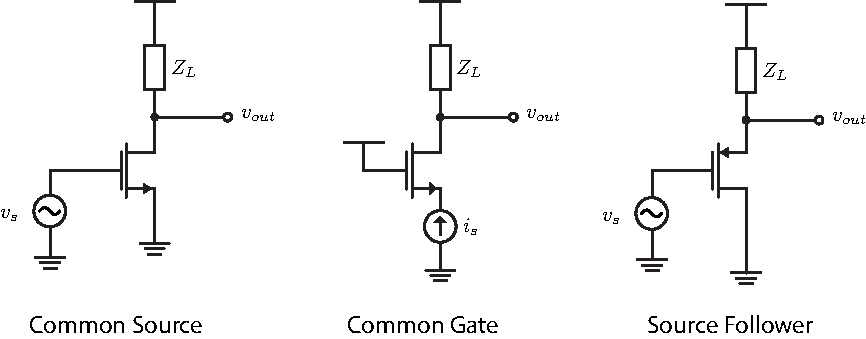
\includegraphics[width=1\columnwidth]{0highZload.pdf}
\caption{High voltage gain amplifiers require a high load impedance $Z_L$.}
\label{fig:0highZload.pdf}
\end{figure}
%%%%%%%%%%%%%%%%%%%%%%%%%%%%%%%%%%%%%%%%%%%%
In each amplifier shown in Fig.~\ref{fig:0highZload.pdf}, to maximize gain we should maximize the load impedance $Z_L$.   Can we just use an arbitrarily large load resistor?  In an IC process technology, resistors are realized either as diffusion regions or using polysilicon films.  The resistance per square is on the order of 100's to 1000's of ohms-per-square, which requires many squares to realize a large resistor, taking up a lot of area.  We are also limited in the minimum width of the resistor, since thinner resistors have limits on maximum current handling capability (due to self-heating) and also experience wider variations from part to part, making the design gain more variable.  But the biggest limitation of all is simply the voltage drop across the resistors, discussed next. 
%%%%%%%%%%%%%%%%%%%%%%%%%%%%%%%%%%%%%%%%%%%%
%             SUBSECTION 13.2.2            %
%%%%%%%%%%%%%%%%%%%%%%%%%%%%%%%%%%%%%%%%%%%%
\subsection{Headroom Limitations}
%%%%%%%%%%%%%%%%%%%%%%%%%%%%%%%%%%%%%%%%%%%%
%                 FIGURE                   %
%%%%%%%%%%%%%%%%%%%%%%%%%%%%%%%%%%%%%%%%%%%%
\begin{figure}[tb]
\centering
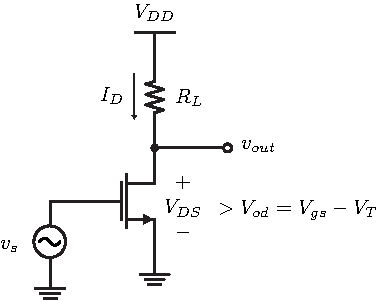
\includegraphics[scale=1]{1cs_headroom.pdf}
\caption{To maximize voltage gain, the transistor should operate in the saturation (or forward-active) region, which means $V_{DS} > V_{od}$ ($V_{CE} > V_{CE,sat}$), which places limits on how large we can make $R_L$ for a fixed bias current.}
\label{fig:1cs_headroom.pdf}
\end{figure}
%%%%%%%%%%%%%%%%%%%%%%%%%%%%%%%%%%%%%%%%%%%%
To keep the transistor in saturation requires $V_{DS} > V_{od}$ (the over-drive voltage, $V_{GS} - V_T$).  For a fixed bias current, if we increase $R_L$, eventually we squash the transistor and it goes from the saturation region to the triode region, and the gain of the circuit is compromised.  This is illustrated in Fig.~\ref{fig:1cs_headroom.pdf}.  One solution is to use a larger $V_{DD}$, but in practice this solution is hard to implement because each generation of IC technology has a voltage supply limit.  For example, today's nanoscale transistors can only tolerate $\sim 1$V of voltage supply due to the thin oxides in the devices.  Even ``thick oxide" devices, available for I/O\footnote{Iinput/output devices are used for driving external loads and receiving inputs from the outside of the chip.}, typically work at a maximum voltage of 2.5V or 3.3V (these voltage levels are standardized).
%%%%%%%%%%%%%%%%%%%%%%%%%%%%%%%%%%%%%%%%%%%%
%             SUBSECTION 13.2.3            %
%%%%%%%%%%%%%%%%%%%%%%%%%%%%%%%%%%%%%%%%%%%%
\subsection{Achieving High Gain}
%%%%%%%%%%%%%%%%%%%%%%%%%%%%%%%%%%%%%%%%%%%%
%                 FIGURE                   %
%%%%%%%%%%%%%%%%%%%%%%%%%%%%%%%%%%%%%%%%%%%%
\begin{figure}[tb]
\centering
\begin{tabular}{cc}
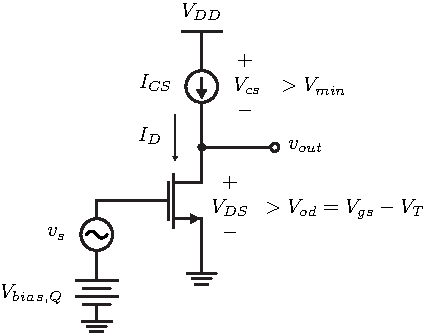
\includegraphics[width=.45\columnwidth]{2cs_current_mirror_load.pdf} &
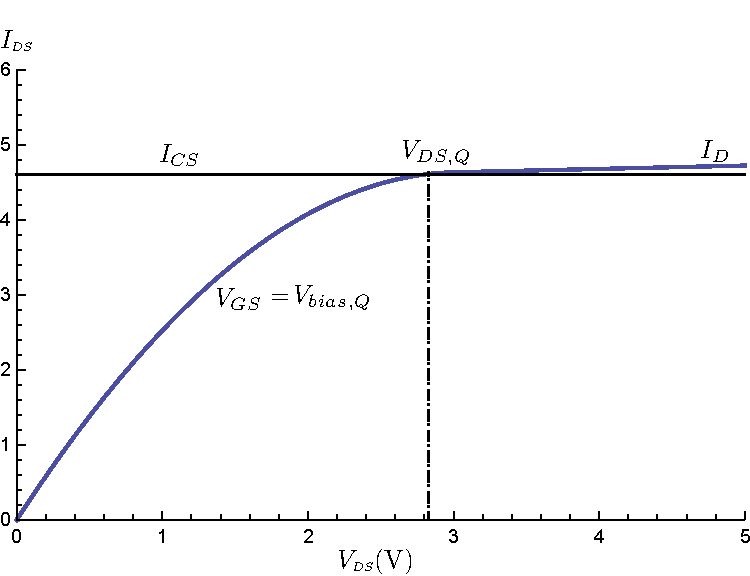
\includegraphics[width=.45\columnwidth]{mos_output_voltage.pdf}\\
(a) & (b)\\
\end{tabular}
\caption{(a) An ideal current source load results in the maximum gain for any bias current.  An ideal current source does not dictate the output voltage, just the current.  Note that $V_{bias,Q}$ determines the transistor operating point, which should match $I_{CS}$.  (b) The actual output voltage is determined by the transistor $I_{DS}$-$V_{DS}$ curve.}
\label{fig:2cs_current_mirror_load.pdf}
\end{figure}
%%%%%%%%%%%%%%%%%%%%%%%%%%%%%%%%%%%%%%%%%%%%
What if someone handed you a current source?  Then you could use it to bias the transistor, as shown in Fig.~\ref{fig:2cs_current_mirror_load.pdf}, and since an ideal current source has infinite output resistance, it would maximize the gain while supporting any value of $V_{DS}$.  Unfortunately ideal current sources don't exist, but we could build one from a transistor with a fixed gate bias.  But how should we generate the correct bias voltage?  We'll answer this question by first considering the wrong approach.
%%%%%%%%%%%%%%%%%%%%%%%%%%%%%%%%%%%%%%%%%%%%
%             SUBSECTION 13.2.4            %
%%%%%%%%%%%%%%%%%%%%%%%%%%%%%%%%%%%%%%%%%%%%
\subsection{Transistor Current Source}
%%%%%%%%%%%%%%%%%%%%%%%%%%%%%%%%%%%%%%%%%%%%
%                 FIGURE                   %
%%%%%%%%%%%%%%%%%%%%%%%%%%%%%%%%%%%%%%%%%%%%
\begin{figure}[tb]
\centering
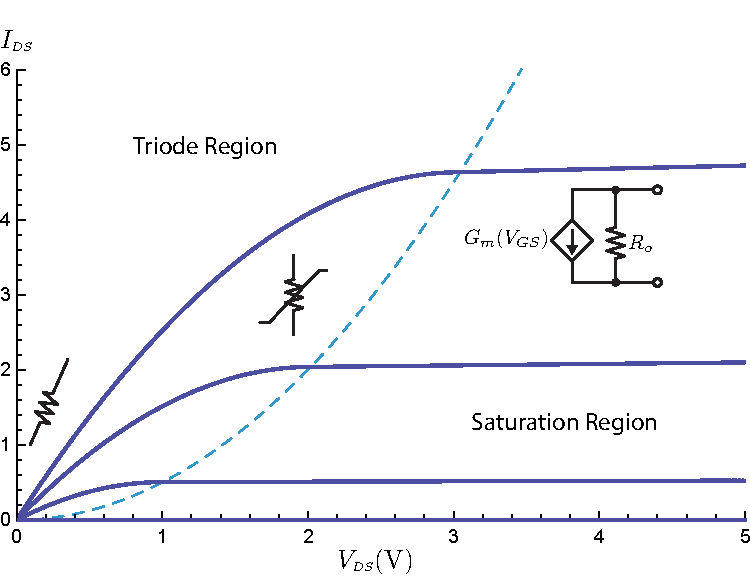
\includegraphics[width=.75\columnwidth]{mos_building_block.pdf}
\caption{An MOS transistor in the saturation region, or a BJT in the forward active region, has nearly constant current as a function of $V_{DS}$, making it a suitable proxy for an ideal current source if the output voltage does not go too low (or high for a PMOS transistor).  The gate voltage (base voltage) must be held constant at the appropriate bias voltage.}
\label{fig:mos_building_block.pdf}
\end{figure}
%%%%%%%%%%%%%%%%%%%%%%%%%%%%%%%%%%%%%%%%%%%%
A transistor biased in saturation with $V_{GS} = \text{constant}$ is effectively a decent current source, as shown in the $I$-$V$ curve in Fig.~\ref{fig:mos_building_block.pdf}.  Even though the transistor is a dependent current source, the main source of dependence is the gate voltage, which we would like to hold constant.  The other dependence is the output resistance, which is much smaller, and results in non-zero slope in the $I$-$V$ curve. 
%%%%%%%%%%%%%%%%%%%%%%%%%%%%%%%%%%%%%%%%%%%%
%             SUBSECTION 13.2.5            %
%%%%%%%%%%%%%%%%%%%%%%%%%%%%%%%%%%%%%%%%%%%%
\subsection{Transistor Process / Temperature Variations}
If we simply fix the $V_{GS}$ value to realize a specific current, we are designing a current source that will have a very unpredictable output current.  For example, if the temperature varies, the threshold voltage changes, and so will the current.  Also, if we fix the gate bias value based on a model, then in real applications we'll find that every transistor is a bit different from the model from natural statistical variations (in doping levels and geometry, especially for small transistors), and so the output current will be a random variable with a large variance.  To keep the variance low, we should use another strategy, which is to observe that while two arbitrary transistors are not well matched, two transistors sitting right next to each other, or better yet two ``inter-digitated transistors" (how this is done will be explained in Sect.~\ref{sec:interdigitate}), will behave very similarly. So the strategy should be to use one transistor to generate the $V_{GS}$ for the other.
%%%%%%%%%%%%%%%%%%%%%%%%%%%%%%%%%%%%%%%%%%%%%%%%%%%%%%%%%%%%%%%%%%%%%%%%%%%%%%%%%%%%%%%%
%%%%%%%%%%%%%%%%%%%%%%%%%%%%%%%%%%%%%%%%%%%%%%%%%%%%%%%%%%%%%%%%%%%%%%%%%%%%%%%%%%%%%%%%
%                                   SECTION 13.3                                       %
%%%%%%%%%%%%%%%%%%%%%%%%%%%%%%%%%%%%%%%%%%%%%%%%%%%%%%%%%%%%%%%%%%%%%%%%%%%%%%%%%%%%%%%%
%%%%%%%%%%%%%%%%%%%%%%%%%%%%%%%%%%%%%%%%%%%%%%%%%%%%%%%%%%%%%%%%%%%%%%%%%%%%%%%%%%%%%%%%
\section{The Basic Current Mirror}
%%%%%%%%%%%%%%%%%%%%%%%%%%%%%%%%%%%%%%%%%%%%
%             SUBSECTION 13.3.1            %
%%%%%%%%%%%%%%%%%%%%%%%%%%%%%%%%%%%%%%%%%%%%
\subsection{Diode Connected Device}
%%%%%%%%%%%%%%%%%%%%%%%%%%%%%%%%%%%%%%%%%%%%
%                 FIGURE                   %
%%%%%%%%%%%%%%%%%%%%%%%%%%%%%%%%%%%%%%%%%%%%
\begin{figure}[tb]
\centering
\begin{tabular}{cc}
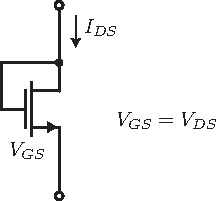
\includegraphics[scale=1]{3mos_diode.pdf} &
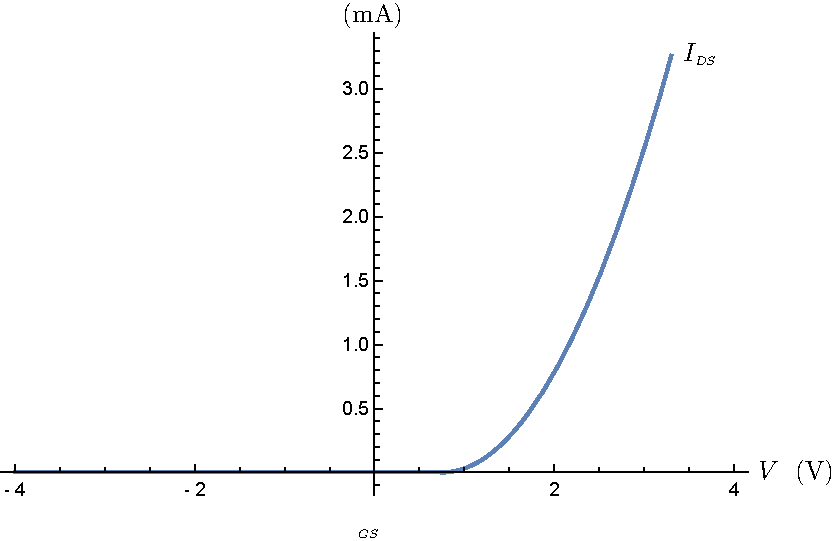
\includegraphics[width=.5\columnwidth]{ivrect.pdf}\\
(a) & (b)\\
\end{tabular}
\caption{(a) An MOS transistor with gate-drain shorted is known as a ``diode connected" transistor.  It behaves as a non-linear unidirectional conductor, similar to a diode.  (b) The $I_{DS}$-$V_{GS}$ of a MOS diode is ``rectifying" in that it only allows current to flow in one direction.}
\label{fig:3mos_diode.pdf}
\end{figure}
%%%%%%%%%%%%%%%%%%%%%%%%%%%%%%%%%%%%%%%%%%%%
The diode connected MOS transistor, shown in Fig.~\ref{fig:3mos_diode.pdf}, is a two-terminal device.  It is never in the triode region because of the gate-drain connection.  Since $V_{DS} = V_{GS}$, as long as $V_{GS}$ is over the threshold voltage, then drain-source voltage is a threshold voltage away from saturation, since $V_{DS} = V_{GS} = V_{dsat} + V_T$.  As we sweep $V_{GS}$ and observe the drain-source current, the transistor goes from ``off" state (below threshold) to the ``on" state.  It's called a diode because of the rectifying action of the the $I$-$V$ relation. Current can pass in one direction, but not the other, similar to a pn-junction diode.  The curve is not exponential, though, since the MOS device $I$-$V$ relation is quadratic.  If we pass a known current into a diode, the $V_{GS}$ value will be well-defined and equal to the value needed to generate the current. It's like an inverse function, that takes a current and generates the correct $V_{GS}$:
    \begin{equation}
        V_{GS} = V_T + \sqrt{\frac{2 I_{DS}}{\frac{W}{L} \mu C_{ox}}} = V_T + V_{od}
    \end{equation}
If the current injected into the device is very low, $V_{od}$ will be low and the diode $V_{GS}$ will be approximately $V_T$.  In general for any current, the $V_{GS}$ generated can be used to bias a second transistor into the same current. 
%%%%%%%%%%%%%%%%%%%%%%%%%%%%%%%%%%%%%%%%%%%%
%             SUBSECTION 13.3.2            %
%%%%%%%%%%%%%%%%%%%%%%%%%%%%%%%%%%%%%%%%%%%%
\subsection{Diode Connected -- Small-Signal Model}
%%%%%%%%%%%%%%%%%%%%%%%%%%%%%%%%%%%%%%%%%%%%
%                 FIGURE                   %
%%%%%%%%%%%%%%%%%%%%%%%%%%%%%%%%%%%%%%%%%%%%
\begin{figure}[tb]
\centering
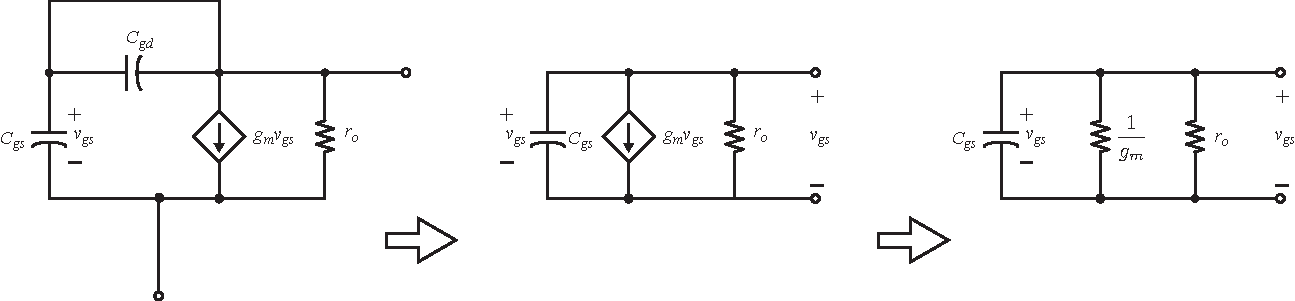
\includegraphics[width=\columnwidth]{4mos_diode_ss.pdf}
\caption{The small-signal model of a diode connected MOS transistor.  Notice that the model is simply a conductance when the gate-drain are shorted, as shown on the right.}
\label{fig:4mos_diode_ss.pdf}
\end{figure}
%%%%%%%%%%%%%%%%%%%%%%%%%%%%%%%%%%%%%%%%%%%%
We can derive the small-signal model by shorting out the drain-gate in the hybrid-$\pi$ model, shown in Fig.~\ref{fig:4mos_diode_ss.pdf}.  Note that a $g_m$ generator with its controlling terminals connected to the $g_m$ is more simply a conductor.  From the perspective of the driving terminal, the MOS diode is just a conductance.
%%%%%%%%%%%%%%%%%%%%%%%%%%%%%%%%%%%%%%%%%%%%
%             SUBSECTION 13.3.3            %
%%%%%%%%%%%%%%%%%%%%%%%%%%%%%%%%%%%%%%%%%%%%
\subsection{The Integrated ``Current Mirror"}
%%%%%%%%%%%%%%%%%%%%%%%%%%%%%%%%%%%%%%%%%%%%
%                 FIGURE                   %
%%%%%%%%%%%%%%%%%%%%%%%%%%%%%%%%%%%%%%%%%%%%
\begin{figure}[tb]
\centering
\begin{tabular}{cc}
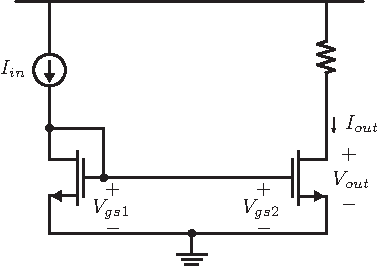
\includegraphics[scale=1]{5mirror_105.pdf} &
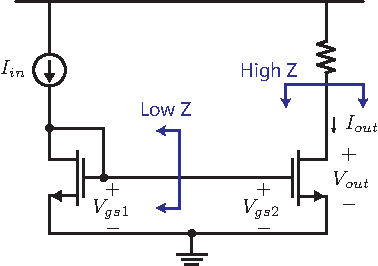
\includegraphics[scale=1]{5bmirror_105.pdf}\\
(a) & (b)\\
\end{tabular}
\caption{(a) An NMOS current mirror has an output current $I_{out}$ that is a ``mirror copy" of $I_{in}$.  (b) The mirror has low impedance on the ``diode" side and high impedance at the output.} \label{fig:5mirror_105.pdf}
\end{figure}
%%%%%%%%%%%%%%%%%%%%%%%%%%%%%%%%%%%%%%%%%%%%
With the MOS diode as a voltage reference, we can build a ``current mirror", shown in Fig.~\ref{fig:5mirror_105.pdf}a.  Since M1 and M2 have the same $V_{GS}$, as long as M2 is in saturation, they will carry approximately the same current.  If we neglect CLM ($\lambda = 0$), then the drain currents would be equal. Since $\lambda$ is small, the currents will nearly mirror one another even if $V_{out}$ is not equal to $V_{gs1}$. We say that the current $I_{in}$ is mirrored into $I_{out}$. Notice that the mirror works for small and large signals!
%%%%%%%%%%%%%%%%%%%%%%%%%%%%%%%%%%%%%%%%%%%%
It's important to note that the diode side of the current is low impedance, due to the diode connection, as shown in Fig.~\ref{fig:5mirror_105.pdf}b.  On the other hand, from the drain of M2 the circuit presents a high impedance, thereby behaving like a current source.
%%%%%%%%%%%%%%%%%%%%%%%%%%%%%%%%%%%%%%%%%%%%
%             SUBSECTION 13.3.4            %
%%%%%%%%%%%%%%%%%%%%%%%%%%%%%%%%%%%%%%%%%%%%
\subsection{Current Mirror with Multiplication Ratio} \label{sec:interdigitate}
%%%%%%%%%%%%%%%%%%%%%%%%%%%%%%%%%%%%%%%%%%%%
%                 FIGURE                   %
%%%%%%%%%%%%%%%%%%%%%%%%%%%%%%%%%%%%%%%%%%%%
\begin{figure}[tb]
\centering
\begin{tabular}{cc}
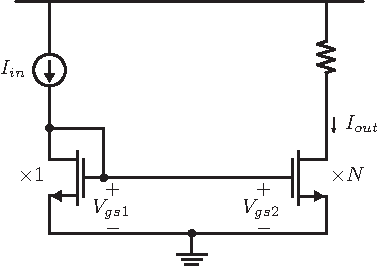
\includegraphics[scale=.8]{6mirror_105_amp.pdf} &
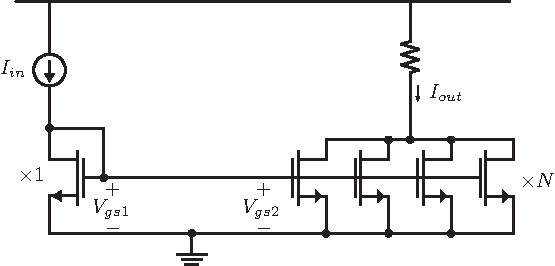
\includegraphics[scale=.8]{6mirror_105_amp_Ncopies.pdf}\\
(a) & (b)\\
\end{tabular}
\caption{A current mirror can be configured to scale the input current by scaling the transistor dimensions $W/L$, or more preferably (b) the $W$ or the transistor count, using parallel devices to realize a larger $W$.}
\label{fig:6mirror_105_amp.pdf}
\end{figure}
%%%%%%%%%%%%%%%%%%%%%%%%%%%%%%%%%%%%%%%%%%%%
With some minor modifications, we can generate a mirror that scales the input current up or down. The input and output currents are related as follows:
    \begin{equation}
        {I_{IN}} = k\frac{{{W_1}}}{{{L_1}}}{({V_{GS1}} - {V_T})^2}
    \end{equation}
    \begin{equation}
        {I_{OUT}} = k\frac{{{W_2}}}{{{L_2}}}{({V_{GS2}} - {V_T})^2}
    \end{equation}
The circuit connections forces the two transistors to operate at the same $V_{GS}$.  Assuming that they have the same threshold voltage (which is a good assumption if the transistors are nearby and laid-out together):
    \begin{equation}
        {V_{GS1}} = {V_{GS2}}
    \end{equation}
Which allows us to write:
    \begin{equation}
        {I_{OUT}} = k\frac{{{W_2}}}{{{L_2}}}{({V_{GS2}} - {V_T})^2} = {I_{IN}}\frac{{{W_2}/{L_2}}}{{{W_1}/{L_1}}} = N \cdot {I_{IN}}
    \end{equation}
In practice we prefer not to scale $L$, but rather the transistor widths $W$ to achieve the desired scaling ratio $N$ (unless $N$ is very large, then a combination of the both $L$ and $W$ will be scaled).  This is because the transistor threshold voltage and other parameters will vary with $L$, and it's best to match the two mirror transistors as much as possible, so they should have the same channel length.  In fact, the most accurate mirror is realized by inter-digitating two transistors, effectively connecting multiple unit transistors in parallel (see Fig.~\ref{fig:6mirror_105_amp.pdf}b), or better yet using multiple ``fingers" in the layout of the transistors (see Fig.~\ref{fig:mirror_layout}):
    \begin{equation}
        {I_{OUT}} =  {I_{IN}}\frac{W_2}{W_1} = {I_{IN}}\frac{N_2\cdot W_U}{N_1\cdot W_U} = N \cdot {I_{IN}}
    \end{equation}
where $W_U$ is the unit transistor width.  
%%%%%%%%%%%%%%%%%%%%%%%%%%%%%%%%%%%%%%%%%%%%
%                 FIGURE                   %
%%%%%%%%%%%%%%%%%%%%%%%%%%%%%%%%%%%%%%%%%%%%
\begin{figure}[tb]
\centering
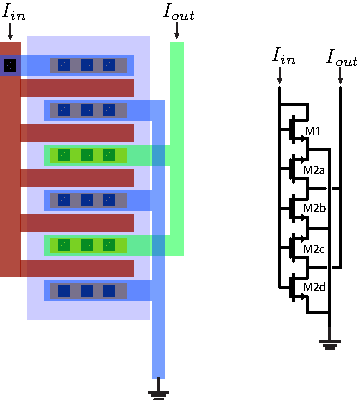
\includegraphics[width=.55\columnwidth]{mirror_layout.pdf} 
\caption{The layout of a 4:1 mirror using 5 unit elements. Note that transistors are abutted and source/drain junctions are shared to maximize matching between the gates, save area and minimize parasitics.  The input transistor is diode connected and the output transistor is split into four fingers.}
\label{fig:mirror_layout}
\end{figure}
%%%%%%%%%%%%%%%%%%%%%%%%%%%%%%%%%%%%%%%%%%%%
%             SUBSECTION 13.3.5            %
%%%%%%%%%%%%%%%%%%%%%%%%%%%%%%%%%%%%%%%%%%%%
\subsection{Current Mirror as Current Source}
%%%%%%%%%%%%%%%%%%%%%%%%%%%%%%%%%%%%%%%%%%%%
%                 FIGURE                   %
%%%%%%%%%%%%%%%%%%%%%%%%%%%%%%%%%%%%%%%%%%%%
\begin{figure}[tb]
\centering
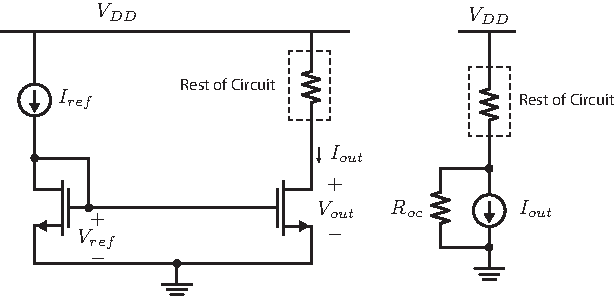
\includegraphics[scale=1]{7mirror_current_source.pdf}
\caption{From the perspective of the ``rest of the circuit" shown, the current mirror appears like an ideal current source with output impedance $R_{oc}$.}
\label{fig:7mirror_current_source.pdf}
\end{figure}
%%%%%%%%%%%%%%%%%%%%%%%%%%%%%%%%%%%%%%%%%%%%
As shown in Fig.~\ref{fig:7mirror_current_source.pdf}, a current mirror acts like a current source to the rest of the circuit as long as the transistor M2 remains in saturation, where it has high output resistance.  Of course, there's a slight problem in that we need another voltage reference $I_{ref}$ to make this work.  The idea is that we generate one very accurate current reference using techniques that we'll discuss in Section~\ref{sec:Ireference}, and this current reference can be mirrored around to various parts of the circuit using mirrors.  
%%%%%%%%%%%%%%%%%%%%%%%%%%%%%%%%%%%%%%%%%%%%
%             SUBSECTION 13.3.6            %
%%%%%%%%%%%%%%%%%%%%%%%%%%%%%%%%%%%%%%%%%%%%
\subsection{Small-Signal Resistance of Current Source}
%%%%%%%%%%%%%%%%%%%%%%%%%%%%%%%%%%%%%%%%%%%%
%                 FIGURE                   %
%%%%%%%%%%%%%%%%%%%%%%%%%%%%%%%%%%%%%%%%%%%%
\begin{figure}[tb]
\centering
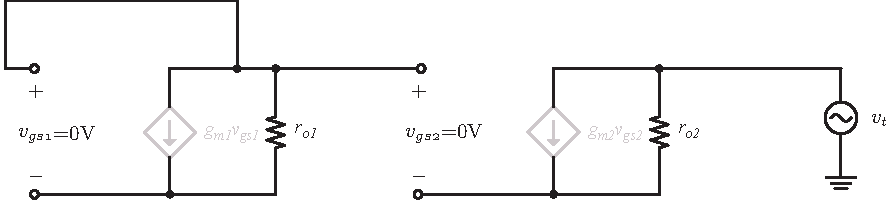
\includegraphics[scale=0.95]{8mirror_small_signal.pdf}
\caption{Current mirror small-signal model.  Transconductors are open-circuit (off) since the controlling voltages are zero.}
\label{fig:8mirror_small_signal.pdf}
\end{figure}
%%%%%%%%%%%%%%%%%%%%%%%%%%%%%%%%%%%%%%%%%%%%
The output impedance seen by the load can be calculated using the small-signal model shown in Fig.~\ref{fig:8mirror_small_signal.pdf}.  Use a test generator $v_t$ and find the current draw from the source.  Note that M1 is not driven by a source because $I_{ref}$ is DC and so an open circuit in the small-signal model.  Thus without a source, M1 is effectively driven with zero $v_{gs}$ and has no output, pulling the $v_{gs}$ of both transistors to ground.  Thus M2's dependent $g_m$ is zero, and the only current draw is from $r_{o,2}$.
%%%%%%%%%%%%%%%%%%%%%%%%%%%%%%%%%%%%%%%%%%%%%%%%%%%%%%%%%%%%%%%%%%%%%%%%%%%%%%%%%%%%%%%%
%%%%%%%%%%%%%%%%%%%%%%%%%%%%%%%%%%%%%%%%%%%%%%%%%%%%%%%%%%%%%%%%%%%%%%%%%%%%%%%%%%%%%%%%
%                                   SECTION 13.4                                       %
%%%%%%%%%%%%%%%%%%%%%%%%%%%%%%%%%%%%%%%%%%%%%%%%%%%%%%%%%%%%%%%%%%%%%%%%%%%%%%%%%%%%%%%%
%%%%%%%%%%%%%%%%%%%%%%%%%%%%%%%%%%%%%%%%%%%%%%%%%%%%%%%%%%%%%%%%%%%%%%%%%%%%%%%%%%%%%%%%
\section{Improved Current Source:  The Cascode Mirror}
%%%%%%%%%%%%%%%%%%%%%%%%%%%%%%%%%%%%%%%%%%%%
%             SUBSECTION 13.4.1            %
%%%%%%%%%%%%%%%%%%%%%%%%%%%%%%%%%%%%%%%%%%%%
\subsection{Improved Current Sources}
The goal is to increase $R_{out}$ of the basic current mirror.  To get a hint about how to proceed, let's look at \textit{amplifier} output resistance results to see topologies that boost resistance.  The output impedance of the common-gate stage is boosted by placing a resistor in the source of the amplifier.  Likewise, the same is true of a common-source amplifier with source degeneration.  The same approach can be used to boost the output impedance of a mirror, as shown in Fig.~\ref{fig:9mirror_Rs.pdf}.
%%%%%%%%%%%%%%%%%%%%%%%%%%%%%%%%%%%%%%%%%%%%
%                 FIGURE                   %
%%%%%%%%%%%%%%%%%%%%%%%%%%%%%%%%%%%%%%%%%%%%
\begin{figure}[tb]
\centering
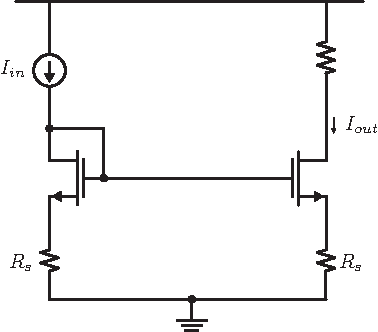
\includegraphics[scale=1]{9mirror_Rs.pdf}
\caption{Adding resistors in the source of a current mirror can be used to boost the output impedance at the cost of reducing the voltage headroom.  Note that the output impedance is boosted by a factor $g_m R_s$, rather than the additive factor of $R_s$, which would be true if the resistor were placed on the drain side.}
\label{fig:9mirror_Rs.pdf}
\end{figure}
%%%%%%%%%%%%%%%%%%%%%%%%%%%%%%%%%%%%%%%%%%%%
%             SUBSECTION 13.4.2            %
%%%%%%%%%%%%%%%%%%%%%%%%%%%%%%%%%%%%%%%%%%%%
\subsection{Effect of Source Degeneration}
%%%%%%%%%%%%%%%%%%%%%%%%%%%%%%%%%%%%%%%%%%%%
%                 FIGURE                   %
%%%%%%%%%%%%%%%%%%%%%%%%%%%%%%%%%%%%%%%%%%%%
\begin{figure}[tb]
\centering
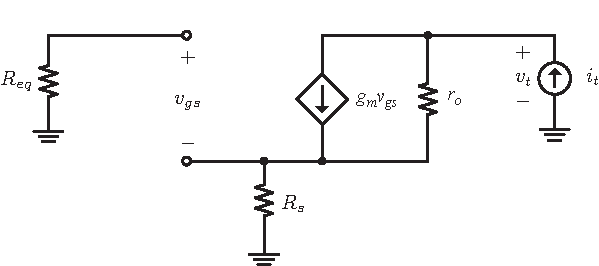
\includegraphics[scale=1]{10mirrror_Rs_ss.pdf}
\caption{Small-signal model of improved output impedance mirror utilizing source resistance $R_s$.} \label{fig:10mirrror_Rs_ss.pdf}
\end{figure}
%%%%%%%%%%%%%%%%%%%%%%%%%%%%%%%%%%%%%%%%%%%%
Let's analyze the small-signal model of the mirror with $R_S$.  We focus on the output side, or transistor M2, and model the input side as a Thevenin equivalent $R_{eq}$ resistance, since there are no sources on the left side.  We inject a test current $i_t$ and measure the voltage developed across $i_t$:
    \begin{equation}
        {v_t} = ({i_t} - {g_m}{v_{gs}}){r_o} + {v_{{R_S}}}
    \end{equation}
First let's note that the current $i_t$ flows through $R_S$ as it returns through the source, which implies the voltage across $R_S$ is given by:
    \begin{equation}
        {v_{{R_S}}} = {i_t}{R_S}
    \end{equation}
The key observation is that the current flowing in $R_S$ generates a source-gate voltage on the transistor:
    \begin{equation}
        {v_{gs}} = - {v_{{R_S}}}
    \end{equation}
which in turn creates a current through $g_m$:
    \begin{equation}
        {v_t} = ({i_t} + {g_m}{R_S}{i_t}){r_o} + {i_t}{R_S}
    \end{equation}
Collecting terms, we find that the output impedance is given by
    \begin{equation}
        {R_o} = \frac{{{v_t}}}{{{i_t}}} = \left( {1 + {g_m}{R_S}} \right){r_o}
    \end{equation}
The output impedance is boosted by factor $(1 + {g_m}{R_S})$ compared to a simple mirror. How would you scale the output current?  If we use the same approach as before, we need to ensure that we scale the resistance as well:
    \begin{equation}
        {I_{IN}} = k\frac{{{W_1}}}{{{L_1}}}{({V_G} - {V_S} - {V_T})^2}
    \end{equation}
where
    \begin{equation}
        {V_S} = {I_{IN}}{R_S}
    \end{equation}
To keep $V_S$ the same, if $I_{OUT}$ is $N$ times larger, then $R_S$ should be $N$ times smaller. 
%%%%%%%%%%%%%%%%%%%%%%%%%%%%%%%%%%%%%%%%%%%%
%             SUBSECTION 13.4.3            %
%%%%%%%%%%%%%%%%%%%%%%%%%%%%%%%%%%%%%%%%%%%%
\subsection{Cascode (or Stacked) Current Source}
%%%%%%%%%%%%%%%%%%%%%%%%%%%%%%%%%%%%%%%%%%%%
%                 FIGURE                   %
%%%%%%%%%%%%%%%%%%%%%%%%%%%%%%%%%%%%%%%%%%%%
\begin{figure}[tb]
\centering
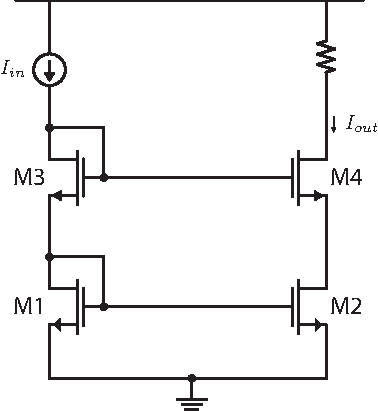
\includegraphics[scale=1]{12mirror_cascode.pdf}
\caption{An improved ``cascode" or stacked current mirror.}
\label{fig:12mirror_cascode.pdf}
\end{figure}
%%%%%%%%%%%%%%%%%%%%%%%%%%%%%%%%%%%%%%%%%%%%
The stacked current mirror, commonly known as the Cascode Current Mirror, is shown in Fig.~\ref{fig:12mirror_cascode.pdf}.  Notice that $V_{GS2}$ is held constant like a normal mirror but now $V_{DS2}$ is also held  approximately constant by M3/M4, making the output current variation much smaller than a single transistor. 
%%%%%%%%%%%%%%%%%%%%%%%%%%%%%%%%%%%%%%%%%%%%
We can easily compute the boost in output impedance by noting that $R_S = r_{o1}$ as far as transistor M4 is concerned: 
    \begin{equation}
        {R_o} \approx \left( {1 + {g_{m2}}{R_S}} \right){r_{o2}} = \left( {1 + {g_{m2}}{r_{o1}}} \right){r_{o2}}
    \end{equation}
Which is approximately $g_m r_o$ times larger than a simple mirror:
    \begin{equation}
        {R_o} \approx {g_{m1}}r_{o1} r_{o2} \gg {r_o}
    \end{equation}
%%%%%%%%%%%%%%%%%%%%%%%%%%%%%%%%%%%%%%%%%%%%
%             SUBSECTION 13.4.4            %
%%%%%%%%%%%%%%%%%%%%%%%%%%%%%%%%%%%%%%%%%%%%
\subsection{Drawback of Cascode Current Source}
Like all good things, there's a catch.  The minimum output voltage to keep all transistors in saturation increases, as shown in Fig.~\ref{fig:mirrors_vmin}.  For a basic current mirror, we can go all the way down to $V_{od}$ and keep M2 in saturation.  When we introduce $R_S$, we have to account for the extra $I_{OUT} R_S$ voltage drop.  With a cascode, the minimum voltage to keep M4 in saturation is given by noting that the source of M4 is biased by M3:
    \begin{equation}
        V_{S,4} = V_{G,4} - V_{GS,4}
        \label{eq:cascodesource}
    \end{equation}
The gate of transistor M4 is basically the $V_{GS}$ of M1 and M3:
    \begin{equation}
        V_{G,4} = V_{GS,1} + V_{GS,3} = 2 V_T + 2 V_{od}
        \label{eq:cascodevgs}
    \end{equation}
To arrive at the right-hand-side of Eq.~\ref{eq:cascodevgs}, we assume all devices have the same $V_T$ and size, so the over-drive voltages are equal.  Since the $V_{GS,4} = V_T + V_{od}$, we can write Eq.~\ref{eq:cascodesource}
    \begin{equation}
        V_{S,4} = V_{G,4} - V_{GS,4}   = 2 V_T + 2 V_{od} - ( V_T + V_{od} ) = V_T + V_{od}
    \end{equation}
Now the minimum $V_{DS,4} = V_{od}$ implies that the cascode mirror has a minimum operating voltage of
    \begin{equation}
        V_{min} = V_T + 2 V_{od}
    \end{equation}
This can be quite a large voltage penalty compared to a simple mirror, but an easy solution is to bias the gate of M4 with $V_T + 2 V_{od}$ using a separate transistor, shown in Fig.~ \label{fig:cascode_hiswing}.  The transistor overdrive voltage is twice as large by scaling the device down by $4\times$.  In a more advanced analog integrated circuits course you'll learn about other ways to realize the ``high swing" cascode.
%%%%%%%%%%%%%%%%%%%%%%%%%%%%%%%%%%%%%%%%%%%%
%                 FIGURE                   %
%%%%%%%%%%%%%%%%%%%%%%%%%%%%%%%%%%%%%%%%%%%%
\begin{figure}[tb]
\centering
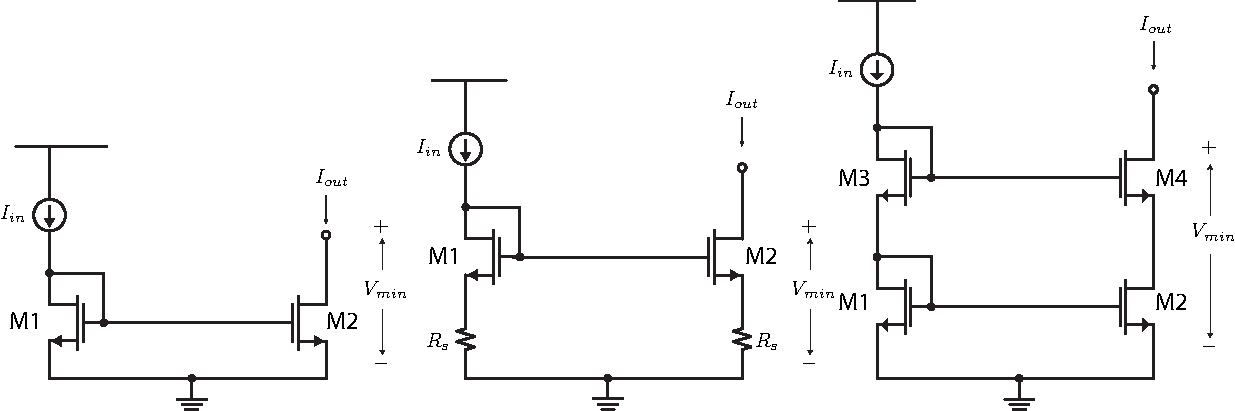
\includegraphics[width=\columnwidth]{mirrors_vmin}
\caption{Comparison of the reduction in the output swing of current mirrors as we improve the output impedance.}
\label{fig:mirrors_vmin}
\end{figure}
%%%%%%%%%%%%%%%%%%%%%%%%%%%%%%%%%%%%%%%%%%%%
%                 FIGURE                   %
%%%%%%%%%%%%%%%%%%%%%%%%%%%%%%%%%%%%%%%%%%%%
\begin{figure}[tb]
\centering
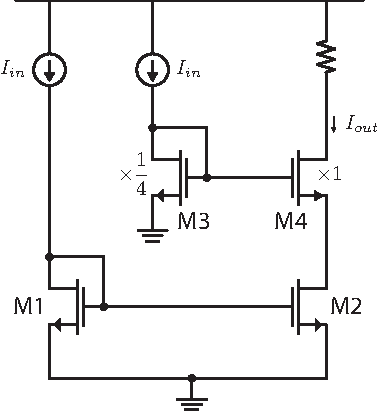
\includegraphics[scale=1]{mirror_cascode_hiswing.pdf}
\caption{To maximize the swing of a cascode mirror, the gate of the top ``cascode" transistor M4 should be biased at $V_T + 2 V_{od}$ to place M2 at the edge of saturation.}
\label{fig:cascode_hiswing}
\end{figure}
%%%%%%%%%%%%%%%%%%%%%%%%%%%%%%%%%%%%%%%%%%%%%%%%%%%%%%%%%%%%%%%%%%%%%%%%%%%%%%%%%%%%%%%%
%%%%%%%%%%%%%%%%%%%%%%%%%%%%%%%%%%%%%%%%%%%%%%%%%%%%%%%%%%%%%%%%%%%%%%%%%%%%%%%%%%%%%%%%
%                                   SECTION 13.5                                       %
%%%%%%%%%%%%%%%%%%%%%%%%%%%%%%%%%%%%%%%%%%%%%%%%%%%%%%%%%%%%%%%%%%%%%%%%%%%%%%%%%%%%%%%%
%%%%%%%%%%%%%%%%%%%%%%%%%%%%%%%%%%%%%%%%%%%%%%%%%%%%%%%%%%%%%%%%%%%%%%%%%%%%%%%%%%%%%%%%
\section{Current Sources and Sinks}
Technically, up to this point we have really been talking about a current ``sink" since the NMOS transistors can only sink current to ground.  What if we need a current ``source"?  The PMOS mirror, shown in Fig.~\ref{fig:18mirror_pmos.pdf}, is exactly the dual of the NMOS mirror, and it simply mirrors a current that is a ``source" from the supply.  In all other aspects, such as the output impedance and scaling, it is identical to the NMOS mirror.  The cascode NMOS mirror can also be replicated and realized in PMOS form. 
%\begin{figure}[tb]
%\centering
%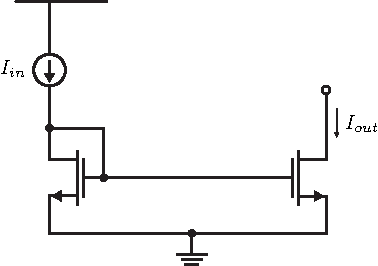
\includegraphics[width=.5\columnwidth]{nmos_source_mirror}
%\caption{nmos source mirror} \label{fig:nmos_source_mirror}
%\end{figure}
%%%%%%%%%%%%%%%%%%%%%%%%%%%%%%%%%%%%%%%%%%%%
%                 FIGURE                   %
%%%%%%%%%%%%%%%%%%%%%%%%%%%%%%%%%%%%%%%%%%%%
\begin{figure}[tb]
\centering
\begin{tabular}{cc}
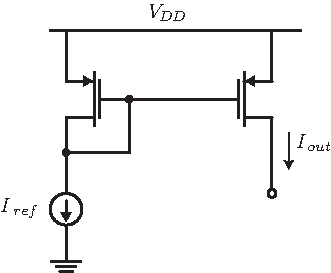
\includegraphics[scale=1]{18mirror_pmos.pdf} &
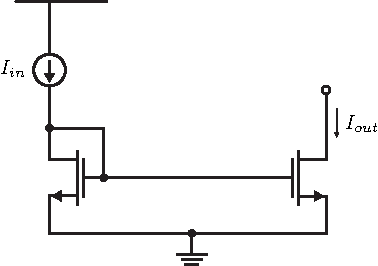
\includegraphics[scale=1]{nmos_source_mirror}\\ 
(a) & (b)\\
\end{tabular}
\caption{(a) A PMOS current source can ``source" a current from supply.  (b) In contrast, an NMOS current can only ``sink" a current to ground.}
\label{fig:18mirror_pmos.pdf}
\end{figure}
%%%%%%%%%%%%%%%%%%%%%%%%%%%%%%%%%%%%%%%%%%%%
%             SUBSECTION 13.5.1            %
%%%%%%%%%%%%%%%%%%%%%%%%%%%%%%%%%%%%%%%%%%%%
\subsection{Generating Multiple Outputs}
One nice observation is that a current mirror can have multiple outputs.  Think of the NMOS diode as a voltage $V_{GS}$ reference.  We can ``export" this reference to multiple transistors in parallel, and each will carry a copy of the reference current, appropriately scaled if desired.  The same reference can then be fed into a PMOS mirror, and the PMOS mirror can likewise produce multiple copies of the current.  These currents can be mirrored to various circuit building blocks as required.  Note that only a single precision $I_{ref}$ is needed to generate dozens or even hundreds of copies.  In section~\ref{sec:Ireference} we'll discuss one simple way to generate this reference that is independent of the supply voltage.
%%%%%%%%%%%%%%%%%%%%%%%%%%%%%%%%%%%%%%%%%%%%
%                 FIGURE                   %
%%%%%%%%%%%%%%%%%%%%%%%%%%%%%%%%%%%%%%%%%%%%
\begin{figure}[tb]
\centering
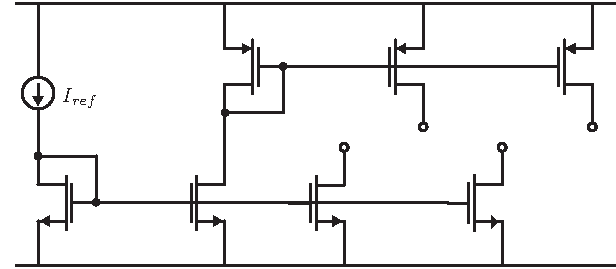
\includegraphics[scale=1]{19current_mirror_multioutput.pdf}
\caption{A precision current reference $I_{ref}$ is fed into this circuit and multiple copies are produced, both as current sinks and sources.  Each current can be scaled appropriately as needed.} \label{fig:19current_mirror_multioutput.pdf}
\end{figure}
%%%%%%%%%%%%%%%%%%%%%%%%%%%%%%%%%%%%%%%%%%%%%%%%%%%%%%%%%%%%%%%%%%%%%%%%%%%%%%%%%%%%%%%%
%%%%%%%%%%%%%%%%%%%%%%%%%%%%%%%%%%%%%%%%%%%%%%%%%%%%%%%%%%%%%%%%%%%%%%%%%%%%%%%%%%%%%%%%
%                                   SECTION 13.6                                       %
%%%%%%%%%%%%%%%%%%%%%%%%%%%%%%%%%%%%%%%%%%%%%%%%%%%%%%%%%%%%%%%%%%%%%%%%%%%%%%%%%%%%%%%%
%%%%%%%%%%%%%%%%%%%%%%%%%%%%%%%%%%%%%%%%%%%%%%%%%%%%%%%%%%%%%%%%%%%%%%%%%%%%%%%%%%%%%%%%
\section{Example:  Source-Follower with Real Current Source}
In this example, we will bias a source-follower (common drain amplifier) using a current mirror, as shown in Fig.~\ref{fig:cd_amp_dc}.  The gate bias voltage $V_{bias,Q}$ needs to be large enough so that the resulting $V_{DS}$ on the drain of the mirror does not ``squash" the transistor into the triode region.  Otherwise there is a lot of flexibility, making this circuit very useful.  In multi-stage amplifiers, the DC bias of the previous stage driving this circuit just needs to be large enough, but the exact value does not matter.
%%%%%%%%%%%%%%%%%%%%%%%%%%%%%%%%%%%%%%%%%%%%
%                 FIGURE                   %
%%%%%%%%%%%%%%%%%%%%%%%%%%%%%%%%%%%%%%%%%%%%
\begin{figure}[tb]
\centering
\begin{tabular}{cc}
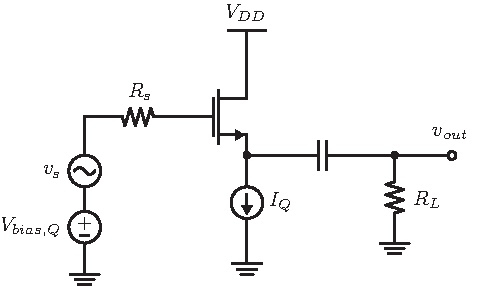
\includegraphics[scale=.8]{cd_amp_dc} &
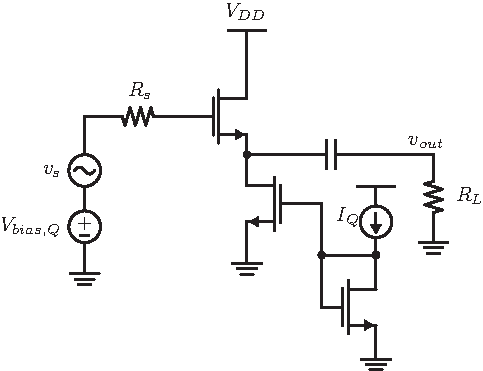
\includegraphics[scale=.8]{cd_amp_dc_mirror}\\
(a) & (b)\\
\end{tabular}
\caption{(a) A MOS source-follower amplifier using an ideal current source is replaced with (b) a current mirror biased amplifier.}
\label{fig:cd_amp_dc}
\end{figure}
%%%%%%%%%%%%%%%%%%%%%%%%%%%%%%%%%%%%%%%%%%%%
%             SUBSECTION 13.6.1            %
%%%%%%%%%%%%%%%%%%%%%%%%%%%%%%%%%%%%%%%%%%%%
\subsection{Common Drain AC Schematic}
The analysis of the AC response using a small-signal model is easily accomplished by simply noting that the current source can be modeled with an effective output resistance $r_{oc}$, as shown in Fig.~\ref{fig:cd_amp_ss_av.pdf}.
%\begin{figure}[tb]
%\centering
%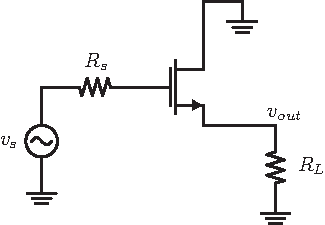
\includegraphics[width=.5\columnwidth]{cd_amp_ac}
%\caption{cd amp ac} \label{fig:cd_amp_ac}
%\end{figure}
%%%%%%%%%%%%%%%%%%%%%%%%%%%%%%%%%%%%%%%%%%%%
%             SUBSECTION 13.6.2            %
%%%%%%%%%%%%%%%%%%%%%%%%%%%%%%%%%%%%%%%%%%%%
\subsection{CD Voltage Gain With Real Current Source}
%%%%%%%%%%%%%%%%%%%%%%%%%%%%%%%%%%%%%%%%%%%%
%                 FIGURE                   %
%%%%%%%%%%%%%%%%%%%%%%%%%%%%%%%%%%%%%%%%%%%%
\begin{figure}[tb]
\centering
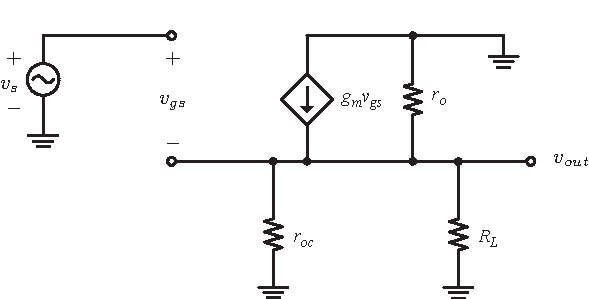
\includegraphics[scale=1]{cd_amp_ss_av.pdf}
\caption{Small-signal model of a source-follower biased with a current mirror, modeled as $r_{oc}$.} \label{fig:cd_amp_ss_av.pdf}
\end{figure}
%%%%%%%%%%%%%%%%%%%%%%%%%%%%%%%%%%%%%%%%%%%%
For an ideal current source, we have
    \begin{equation}
        \frac{{{v_{out}}}}{{{R_L}||{r_o}}} = {g_m}{v_{gs}}
    \end{equation}
and
    \begin{equation}
        \frac{{{v_{out}}}}{{{R_L}||{r_o}}} = {g_m}\left( {{v_{s}} - {v_{out}}} \right)
    \end{equation}
With the NMOS current mirror biasing scheme, all we have to do is add the effect of $r_{oc}$: 
    \begin{equation}
        \frac{{{v_{out}}}}{{{R_L}||{r_o}||r_{oc}}} = {g_m}{v_{gs}}
    \end{equation}
    \begin{equation}
        \frac{{{v_{out}}}}{{{R_L}||{r_o}||r_{oc}}} = {g_m}\left( {{v_{s}} - {v_{out}}} \right)
    \end{equation}
Let $R_{L,eff} =  R_L || r_o || r_{oc}$.   From KCL at the output we have:
    \begin{equation}
        v_{out} = g_m R_{L,eff} (v_s - v_{out} )
    \end{equation}
    \begin{equation}
        v_{out} \left(1 + g_m R_{L,eff} \right) = g_m R_{L,eff} v_s
    \end{equation}
The voltage gain is given by:
    \begin{equation}
        G_v = \frac{v_{out}}{v_s} = \frac{ g_m R_{L,eff}}{ 1 + g_m R_{L,eff}}
    \end{equation}
%%%%%%%%%%%%%%%%%%%%%%%%%%%%%%%%%%%%%%%%%%%%%%%%%%%%%%%%%%%%%%%%%%%%%%%%%%%%%%%%%%%%%%%%
%%%%%%%%%%%%%%%%%%%%%%%%%%%%%%%%%%%%%%%%%%%%%%%%%%%%%%%%%%%%%%%%%%%%%%%%%%%%%%%%%%%%%%%%
%                                   SECTION 13.7                                       %
%%%%%%%%%%%%%%%%%%%%%%%%%%%%%%%%%%%%%%%%%%%%%%%%%%%%%%%%%%%%%%%%%%%%%%%%%%%%%%%%%%%%%%%%
%%%%%%%%%%%%%%%%%%%%%%%%%%%%%%%%%%%%%%%%%%%%%%%%%%%%%%%%%%%%%%%%%%%%%%%%%%%%%%%%%%%%%%%%
\section{Generation of Current References}
\label{sec:Ireference}
%%%%%%%%%%%%%%%%%%%%%%%%%%%%%%%%%%%%%%%%%%%%
%                 FIGURE                   %
%%%%%%%%%%%%%%%%%%%%%%%%%%%%%%%%%%%%%%%%%%%%
\begin{figure}[tb]
\centering
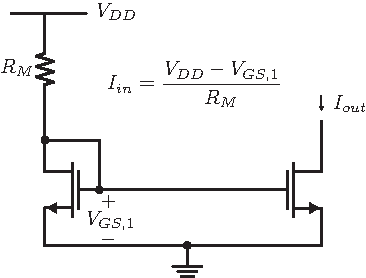
\includegraphics[scale=1]{mirror_resistor.pdf}
\caption{A reference current generator using a resistor.  While it's very simple and convenient, it's supply and temperature dependent.}
\label{fig:iref_gen_rs}
\end{figure}
%%%%%%%%%%%%%%%%%%%%%%%%%%%%%%%%%%%%%%%%%%%%
Up until now we've been ignoring the elephant in the room, which is how to generate the $I_{ref}$ or input current into the mirror.  The simplest way is to simply use a resistor, as shown in Fig.~\ref{fig:iref_gen_rs}.  This solution is simple, but it depends on several parameters that may vary, such as the supply voltage, the transistor $V_T$, and many other parameters such as temperature:  
    \begin{equation}
        I_{ref} = \frac{V_{DD} - V_{GS,1}}{R_M}  
    \end{equation}
Note that $V_{GS,1}$ is a weak function of $I_{ref}$:
    \begin{equation}
        V_{GS,1} = V_T + \sqrt{\frac{2 I_{ref}}{\mu C_{ox} \frac{W}{L}}}
    \end{equation}
We can solve the above equation to obtain $I_{ref}$.
%%%%%%%%%%%%%%%%%%%%%%%%%%%%%%%%%%%%%%%%%%%%
%             SUBSECTION 13.7.1            %
%%%%%%%%%%%%%%%%%%%%%%%%%%%%%%%%%%%%%%%%%%%%
\subsection{Constant \texorpdfstring{$G_m$}{Transconductance} Reference Current}
What we desire is a supply and temperature independent reference current, and to the greatest extent possible, a current that does not depend on transistor parameters, which vary over process and temperature.  There are many clever circuits such as bandgap references that generate precision temperature independent voltages, but in order to generate a current we need a resistor, and unless it's an external precision resistor, there will be variations.  Calibration procedures are needed to tune the currents, a subject beyond the scope of this book.
%%%%%%%%%%%%%%%%%%%%%%%%%%%%%%%%%%%%%%%%%%%%
Here we will not delve into the details of various circuits to build references but instead present one simple and very useful example, the constant-$g_m$ reference generator, shown in Fig.~\ref{fig:constant_gm_ref}.  This example is a particularly good one because it's simple and it builds on the principals we've discussed in this chapter.
%%%%%%%%%%%%%%%%%%%%%%%%%%%%%%%%%%%%%%%%%%%%
%                 FIGURE                   %
%%%%%%%%%%%%%%%%%%%%%%%%%%%%%%%%%%%%%%%%%%%%
\begin{figure}[tb]
\centering
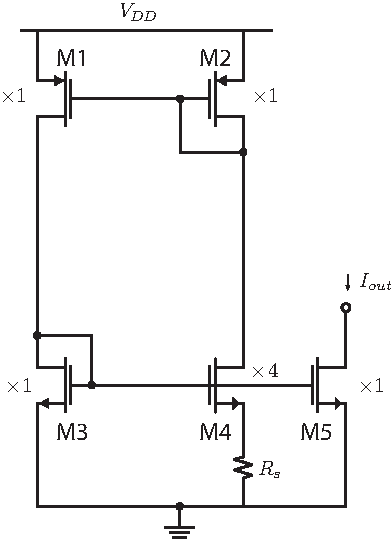
\includegraphics[scale=1]{constant_gm_bias.pdf}
\caption{A reference current generator with an output current that produces a constant $g_m = 1/R_s$, independent of supply voltage and temperature.}
\label{fig:constant_gm_ref}
\end{figure}
%%%%%%%%%%%%%%%%%%%%%%%%%%%%%%%%%%%%%%%%%%%%
With reference to Fig.~\ref{fig:constant_gm_ref}, notice that the PMOS mirror on top enforces current equality between the two branches, as the devices have the same dimensions.  In other words, the currents $I_{D3}$ and $I_{D4}$ must be equal.  The bottom current sources, on the other hand, are not sized the same, and transistor M3 is sized to be exactly $1/4$ smaller than M4.  The voltage across the resistor $R_s$ is given by
    \begin{equation}
        V_{R_S} = \Delta V_{GS} = V_{GS,3} - V_{GS,4}
    \end{equation}
We can express each $V_{GS}$ as a threshold voltage plus an over-drive voltage:
    \begin{equation}
        V_{GS,4} = V_T + \sqrt{\frac{2 I_{D4}}{\mu C_{ox} \left( \frac{W}{L} \right)_4}} = V_T + V_{od4}
    \end{equation}
For device M3, it carries the same current and has 4 times smaller width:
    \begin{equation}
        V_{GS,3} = V_T + \sqrt{\frac{2 I_{D4}}{\mu C_{ox} \left( \frac{1}{4} \frac{W}{L} \right)_4}} = V_T + 2V_{od4}
    \end{equation}
With this observation, the output current of M4 is simply given by
    \begin{equation}
        I_{D4} = \frac{\Delta V_{GS}}{R_S} = \frac{V_{od4}}{R_S}  \label{eq:gm_constant}
    \end{equation}
Substitution of the over-drive voltage leads to the output current:
    \begin{equation}
        I_{D4} = \frac{V_{od4}}{R_S} = \frac{1}{R_S} \sqrt{\frac{2 I_{D4}}{\mu C_{ox} \left( \frac{W}{L} \right)_4}}
    \end{equation}
or
    \begin{equation}
        I_{D4} = \frac{1}{R_S^2} \frac{2}{\mu C_{ox} \left( \frac{W}{L} \right)_4}
    \end{equation}	
Notice that the current $I_{D4}$ does not depend on the supply voltage or the device threshold, so it can be used as a reference current.  If we mirror the current of M3 to another transistor of equal size, it will satisfy Eq.~\ref{eq:gm_constant}.  What is nice about this circuit is that the ratio of current to over-drive voltage, which is related to the transconductance, tracks $R_S$:
    \begin{equation}
        g_{m,5} = \frac{2 I_{D5}}{V_{od5}} = \frac{\cancel{2} I_{D4}}{\cancel{2} V_{od4}} = \frac{1}{R_S} 
    \end{equation}
For this reason, this circuit is known as a constant $g_m$ reference because all transistors biased with this current will have a $g_m$ that is constant and independent of process and temperature.
